\documentclass[conference]{IEEEtran}
\usepackage{cite}
\usepackage{amsmath,amssymb,amsfonts}
\usepackage{graphicx}
\usepackage{textcomp}
\usepackage{xcolor}
\usepackage{multicol}
\usepackage{float}
\usepackage[spanish]{babel}
\usepackage[spanish,vlined,ruled,]{algorithm2e}

\def\BibTeX{{\rm B\kern-.05em{\sc i\kern-.025em b}\kern-.08em
    T\kern-.1667em\lower.7ex\hbox{E}\kern-.125emX}}
\begin{document}

\title{Morphing}
\author{\IEEEauthorblockN{Joaquín Pérez Araya}
\IEEEauthorblockA{\textit{Departamento de Ciencias de la Computación} \\
\textit{Universidad de Chile}\\
Santiago, Chile \\
joaquin.perez.a@ug.uchile.cl}}


\maketitle

\begin{abstract}
	
\end{abstract}
 

\section*{Introducción} % ***Así la cosa no me molesta con los numeritos***
	El morphing es el efecto visual el cual se produce al cambiar una imagen a otra con un efecto de metamorfosis, actualmente se utiliza principalmente para el entretenimiento. En este documento se implementará el algoritmo descrito por Beier-Neely, que consiste en utilizar líneas de correspondencia entre la imagen de partida y la imagen de destino para describir la forma en que la mutación se va a llevar a cabo.
	

\section*{Diseño e Implementación}
	El código implementado se define en 3 partes: El cálculo de un wrapping de una imagen según las líneas de destino y partida, el cálculo del morph total para crear u
\section*{Experimentación}
	Se realizaron pruebas con los siguientes valores para medir los pesos	
	
\section*{Conclusión}
	La técnica implementada de Morphing, es bastante lenta, dado que su tiempo de ejecución aumenta según la cantidad de píxeles, la cantidad de líneas determinadas y la cantidad de imágenes totales que se quieren, sin embargo esto otorga más control a la hora de elegir la forma de cómo se va animando la imagen a lo largo del morphing completo.
	
\begin{thebibliography}{99}
	 \bibitem{Paper} 

\end{thebibliography}

\end{document}

\begin{figure}[H]
    \centering
    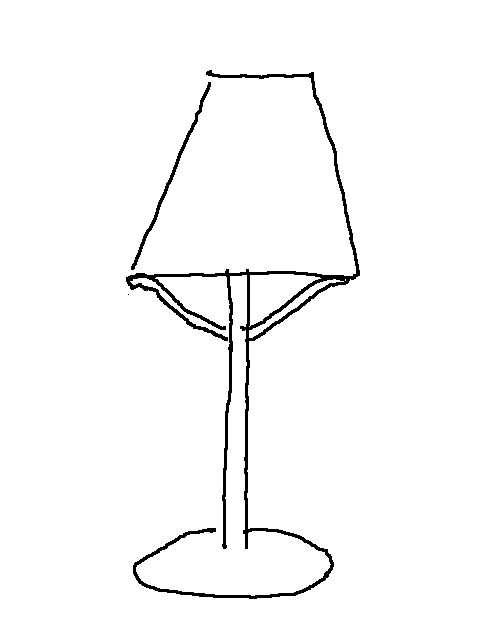
\includegraphics[width=0.95\linewidth]{image/lamps.jpg} \par

\caption{Ejemplo de una posible búsqueda, la imagen de la izquierda representa el dibujo de búsqueda y las de la derecha los resultados esperados.}
\end{figure}